\chapter{Model Evaluation}\label{chap:evaluation}
In working with prediction problems, such as \sti prediction, there are many ways to evaluate how well a classifier (a.k.a. model) performs. In this chapter, we will briefly summarize the evaluation possibilities for a binary classification problem, and discuss why we chose the receiver operating characteristic as our primary metric.

\section{Point metrics for hard decision outputs}
When a classifier produces a hard decision output, i.e. a binary label, we evaluate the classifier using the following metrics.

\subsection{Confusion Matrices}
Generally, the evaluation measures in classification problems form a matrix with the numbers of examples correctly and incorrectly classified for each class, named the confusion matrix. The confusion matrix for a binary classification problem (which has only two classes - positive and negative), is defined by correct and incorrect classifications of positive and negative values. In our case, because we hope to predict \sti, a positive example represents \sti, and a negative example represents staying in the course. Table~\ref{table:confusion_matrix} shows the confusion matrix.
\newcommand\MyBox[2]{
  \fbox{\lower0.75cm
    \vbox to 1.7cm{\vfil
      \hbox to 1.7cm{\hfil\parbox{1.4cm}{#1\\#2}\hfil}
      \vfil}%
  }%
}


\noindent
\renewcommand\arraystretch{1.5}
\setlength\tabcolsep{0pt}

\begin{table*}[htp]
	\centering
	\caption{Dropout Prediction Confusion Matrix}\label{table:confusion_matrix}
	\begin{tabular}{c >{\bfseries}r @{\hspace{0.7em}}c @{\hspace{0.4em}}c @{\hspace{0.7em}}l}
	  \multirow{10}{*}{\parbox{1.1cm}{\bfseries\raggedleft actual\\ value}} & 
	    & \multicolumn{2}{c}{\bfseries Prediction outcome}\\
	  & & \bfseries stopout & \bfseries persist  \\
	  & stopout & \MyBox{True}{Positive} & \MyBox{False}{Negative} \\[2.4em]
	  & persist & \MyBox{False}{Positive} & \MyBox{True}{Negative}  \\
	\end{tabular}
\end{table*}



\begin{itemize}
\item True Positives (TP) are students who we correctly predict as stopping out.
\item False Positives (FP) are students who we predict will \sti, but who stay in the course.
\item False Negatives (FN) are students who we predict will stay in the course, but who actually stopout.
\item True Negatives (TN) are students who we correctly predict as staying in the course.
\end{itemize}

\subsection{Prediction Accuracy}
The simplest evaluation metric is prediction accuracy, which represents how often the classifier correctly predicted an example. A classifier's accuracy is given by $\frac{TN + TP}{FN + FP + TN + TP}$ Prediction accuracy can be applied to any classifier.

When the dataset is skewed towards one label or another, this becomes problematic because the optimal threshold to maximize accuracy favors the more likely label, and the classifier is able to achieve good accuracy by always guessing the more likely choice. This is the case in our dataset, as in any given week, more students stay in the class next week than stopout. If, for example, we are trying to predict one week ahead, and 90\% of students are still in the class next week, then a classifier can achieve 90\% accuracy by simply always predicting that a student will stay in. In addition to this problem, prediction accuracy loses information about the certainty of the answer, as it only outputs the label. For these reasons, prediction accuracy is not the primary metric we use to evaluate our models.

\subsection{Precision and Recall}
In a classification context, precision and recall are additional metrics for how well a classifier performs. Both are defined through equations relating confusion matrix values. 
Precision is given by $\frac{TP}{TP + FP}$. Intuitively, precision represents the accuracy of the classifier among those it classifies as positive examples. In our case, this becomes the fraction of students who were predicted to \sti and actually did leave the course.
Recall is given by $\frac{TP}{TP + FN}$. Intuitively, recall represents how good a classifier is at finding positive examples. In the \sti problem, recall represents the number of stopped out students the classifier is able to identify. A classifier with low recall allows many \sti students to fall through the cracks and escape detection.

For classifiers (such as logistic regression and Hidden Markov Models, classifiers which we use) that give the probability of being in each class, prediction accuracy and the precision recall point require picking a threshold to compare against. For example, for a threshold of 0.7, a classifier could predict that a student will stay in the course if the probability of staying is greater than 0.7. For this reason, this type of metric is called a point metric, or hard decision classification.

\section{Area metrics for soft decisions}
A more comprehensive metric to evaluate classifiers uses every threshold for evaluation. Models that generate a posterior probability estimate for a label are able to do this. An example of an area metric is the precision-recall curve.

\subsection{Precision-recall curve}
Although precision and recall are defined by a confusion matrix, in practice they are often represented as possible precision and recall scores as a classifier sweeps through threshold values. Of course, this sweeping only applies to classifiers which give a probability of being in each class. This produces a precision-recall curve, which graphs possible precision values vs. possible recall values during this threshold sweep. Figure \ref{fig:example_precision_recall} shows an example curve. Each point on the curve represents a threshold. The AUC, or area under the curve, is a simple, one-number metric which represents how well the classifier performs over all thresholds. The precision-recall curve is commonly used in evaluating predictive models.

\begin{figure}[ht!]
  \caption{Example precision-recall curve. The curve was generated using logistic regression on the forum\_only dataset, with a lead of 3 and a lag of 4. This model will be discussed later, but serves here as an example.}\label{fig:example_precision_recall}
  \centering
    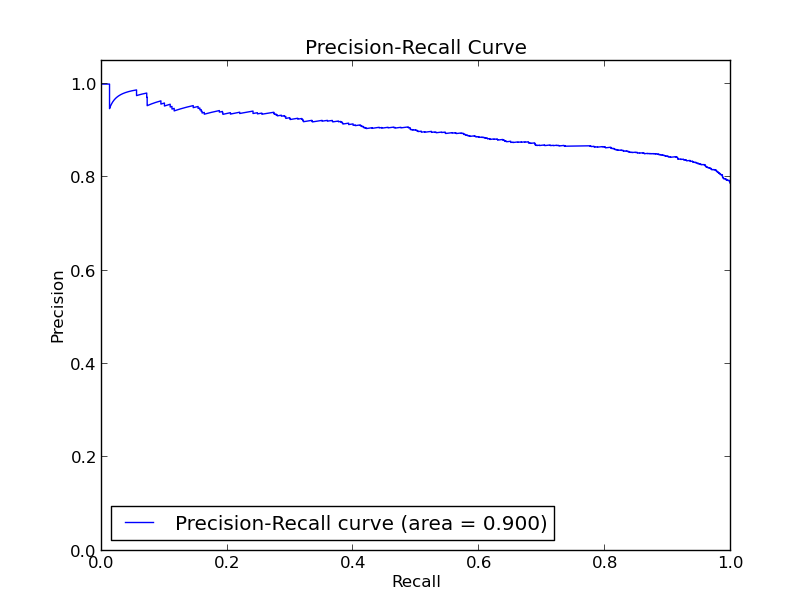
\includegraphics[width=1.0\textwidth]{figures/example_precision_recall.png}
\end{figure}

\subsection{Receiver Operating Characteristic}
Another widely used metric of classifier performance is called the receiver operating characteristic. Like the precision-recall curve, the receiving operating characteristic, or ROC, is a line representing the performance as a classifier sweeps a range of thresholds of decision boundaries. Figure \ref{fig:example_roc} shows an example ROC curve. The ROC curve represents the range of possible probability of False Alarm and probability of Detection values. Both probability of False Alarm (pFA) and probability of Detection (pD) are given by confusion matrix quantities.
pD is equal to $ \frac{TP}{TP + FN}$. This is equivalent to recall, and represents how good a classifier is at finding positive examples.
pFA is equal to $ \frac{FP}{FP + TN}$. This represents how likely a classifier is to mistakenly classify a negative example as a positive one.

\begin{figure}[ht!]
  \caption{Example ROC curve. The curve was generated using logistic regression on the forum\_only dataset, with a lead of 3 and a lag of 4. This model will be discussed later, but serves here as an example.}\label{fig:example_roc}
  \centering
    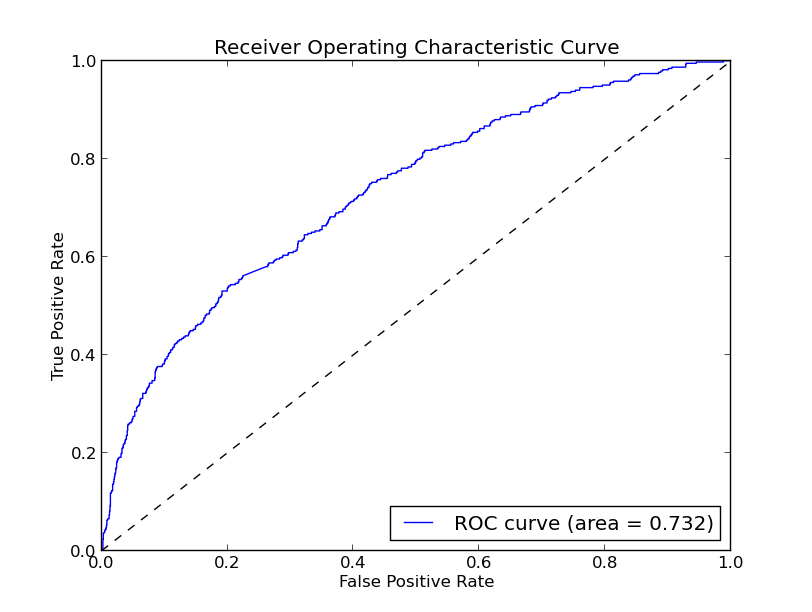
\includegraphics[width=1.0\textwidth]{figures/example_roc.png}
\end{figure}

Like precision and recall, a receiver operating characteristic is useful because it describes a classifier's ability over a wide range of thresholds. Indeed, both are very similar, and in a way equivalently useful for describing a classifier. Which curve to use depends on which value is more important in a prediction problem, which is usually context specific. We choose to use the receiver operating characteristic.

The integral of the ROC curve produces a one-number metric called the area under the curve (AUC). Like the AUC of precision-recall, it concisely describes a classifier, and is the primary metric we use as we compare predictive models. As previously noted, a lot of information is packed into this one number, and thus is a convenient summary of the effectiveness of the model.

\section{Training and Testing}
In order to independently construct and evaluate our models, we divided each cohort's dataset into a mutually exclusive train dataset and test dataset. We chose a 70\% train, 30\% test split, meaning that 70\% of each cohort's data was put into a train dataset, and the remaining was put into a test dataset. In each of our predictive models, we only used the train dataset to build the model, and ultimately evaluated it (using the aforementioned receiver operating characteristic metrics) on the test dataset to determine the model's performance. The test dataset represent previously unknown, sampled data from the population of students, and was never used until the final evaluation of the models.

In order to preserve the distribution of students as best as possible, we aimed to keep the 70/30 split for each stopout week for each cohort. In other words, for each cohort, we split the students who stopped out in week 1 70/30, then split students who stopped out in week 2 70/30, and so on, for each \sti week. In order to achieve that split, we iterated through the overall file, and put students into the appropriate dataset as they appeared so as to constantly keep the 70/30 split over each student. We did so in this way as to not bias the split from the ordering of our file. In other words, neither the train nor test split has a bias towards students who registered for the class earlier. The results are training and testing datasets for each cohort, each of which are proportional to the aggregate cohort in terms of the stopout weeks of the students and student registration times.

\section{Cross validation}
We employed a technique called cross validation in all of our predictive modelling. Cross validation tests a predictive model without the test dataset, in order to gauge when a model might be over-fitting, and to gauge sensitivity in model accuracy from data sensitivity. Some partitions are used in constructing a model, and others are used to evaluate the model's performance. Specifically, we used K-fold cross validation. K-fold cross validation is a commonly used technique which randomly divides the dataset into K folds (or partitions). Cross validation then constructs K models. Each model is constructed using K-1 of the folds, and the model is evaluated using the last unused fold. Figure \ref{fig:cross_validation} shows a diagram of this. K-fold cross validation helps to protect against over-fitting, and provides an alternative and complimentary evaluation metric to the test dataset. Cross validation, and K-fold cross validation are commonly used in practice. In our evaluations, we employ 10 fold cross validation and use the average of the ROC AUC over the folds as another evaluation metric.

\begin{figure}[ht!]
  \caption{The k-fold cross validation partitioning. K models are built, using K-1 folds for model construction and the last fold for model evaluation}\label{fig:cross_validation}
  \centering
    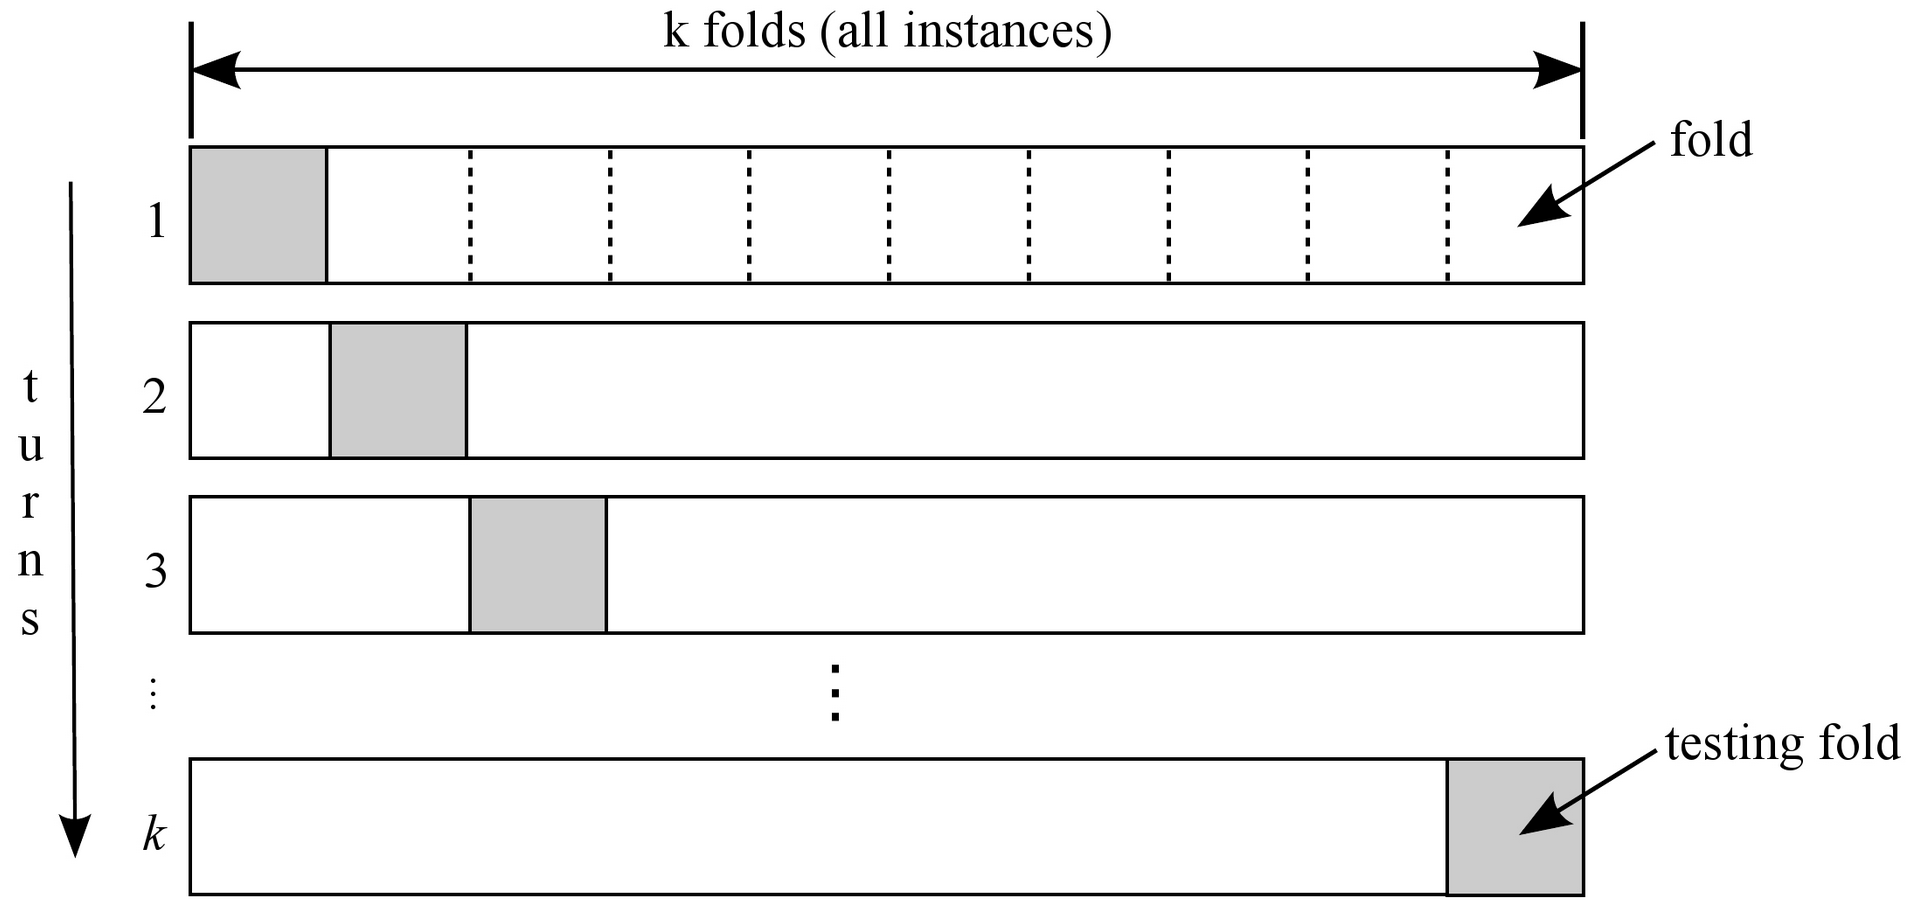
\includegraphics[width=1.0\textwidth]{figures/cross_validation.png}
\end{figure}